\documentclass{article}


% if you need to pass options to natbib, use, e.g.:
%     \PassOptionsToPackage{numbers, compress}{natbib}
% before loading neurips_2023


% ready for submission
% \usepackage{neurips_2023}


% to compile a preprint version, e.g., for submission to arXiv, add add the
% [preprint] option:
\usepackage[preprint]{neurips_2023}


% to compile a camera-ready version, add the [final] option, e.g.:
%     \usepackage[final]{neurips_2023}


% to avoid loading the natbib package, add option nonatbib:
%    \usepackage[nonatbib]{neurips_2023}


\usepackage[utf8]{inputenc} % allow utf-8 input
\usepackage[T1]{fontenc}    % use 8-bit T1 fonts
\usepackage{hyperref}       % hyperlinks
\usepackage{url}            % simple URL typesetting
\usepackage{booktabs}       % professional-quality tables
\usepackage{amsfonts}       % blackboard math symbols
\usepackage{nicefrac}       % compact symbols for 1/2, etc.
\usepackage{microtype}      % microtypography
\usepackage{xcolor}         % colors
\usepackage{graphicx}


\title{CSE 251B Project Final Report}


% The \author macro works with any number of authors. There are two commands
% used to separate the names and addresses of multiple authors: \And and \AND.
%
% Using \And between authors leaves it to LaTeX to determine where to break the
% lines. Using \AND forces a line break at that point. So, if LaTeX puts 3 of 4
% authors names on the first line, and the last on the second line, try using
% \AND instead of \And before the third author name.


\author{%
  Awies Mohammad Mulla\\
  Electrical and Computer Engineering\\
  University of California, San Diego\\
  La Jolla, CA 92093 \\
  \texttt{amulla@ucsd.edu} \\
  % examples of more authors
  % \And
  % Coauthor \\
  % Affiliation \\
  % Address \\
  % \texttt{email} \\
  % \AND
  % Coauthor \\
  % Affiliation \\
  % Address \\
  % \texttt{email} \\
  % \And
  % Coauthor \\
  % Affiliation \\
  % Address \\
  % \texttt{email} \\
  % \And
  % Coauthor \\
  % Affiliation \\
  % Address \\
  % \texttt{email} \\
}


\begin{document}


\maketitle


\begin{abstract}
  Trajectory prediction of the vehicles is one of the major problems in the domain of autonomous navigation.
  The vehicles are identified from the data (Argoverse Dataset used) extracted using sensors like LiDAR, RGBD Stereo Camera 
  which could be then transformed to a pose to be used for the task of trajectory prediction. 
  This is an important problem for safe functioning of various agents simultaneously, along with safety of pedestrians. 
  Not only should the results produced during this step be precise but also the corresponding controller should function 
  with same level accuracy. We will focus on the prediction step in this paper. Over the past years various approaches 
  and algorithm have been introduced to tackle this problem mainly along the lines of unsupervised learning. 
  In this paper we will first introduce the problem and present an analysis on the dataset used for the said task. 
  Moving on to discuss the details of the various algorithms experimented along with the implementation details. 
  Finally, we will present the results produced. Since, this is a milestone report on the project, 
  better results are expected to be presented in the final report by using the approaches whose overview are mentioned 
  in the section future works.

\end{abstract}


\section{Task Description and Background}
For this project we are provided a simplified version of Argoverse Dataset recorded in Miami and Pittsburgh. Original dataset contains
the raw sensor data from the sensors like LiDAR, RGBD Stereo Camera, GPS, IMU, etc. The simplified version of the dataset contains the
2D pose and velocities of the vehicles in the world frame along the information about the neccessary information about the environment like the 
coordinates of the lanes and directions represented by the lane markers. The link to scripts used to generate is \href{https://github.com/awiesmu11a/Autonomous_Vehicle_tracking}{here}. And the
background and applications of this project are mentioned in the abstract.
\\
Our goal is to predict 2D pose of the agent for 30 timestep in the world frame, given the past 19 timestep information (2D pose and velocity in the world frame) of the agent and the
the details of the environment. We are given the coordinates of the lanes on the road, direction of the lane markers (lane norms) and name of the city.
\\
\\
\textbf{Objective:} Minimize the following loss function -
\begin{equation}
    \mathcal{L} = \frac{1}{N}\sum_{i=1}^{N}\sum_{j=1}^{30}\left \| \hat{y}_{i,j} - y_{i,j} \right \|_{2}
\end{equation}
where $\hat{y}_{i,j}$ is the predicted 2D pose of the agent at timestep $j$ for the $i^{th}$ sample and $y_{i,j}$ is the ground truth 2D pose of the agent at timestep $j$ for the $i^{th}$ sample.
$N$ is the number of samples in the dataset. $\hat{y}_{i,j}$ is defined as
\begin{equation}
    \hat{y}_{i,j} = f(x_{i,j:(j-19)}, c_{i})
\end{equation}
where $f(.)$ is the model used for prediction, $x_{i,j:(j-19)}$ is the 2D pose and velocity of the agent at timestep $j$ for the $i^{th}$ sample and $c_{i}$ is the information about the environment for the $i^{th}$ sample.
\\
\\
The model defined above can potentially solve other tasks apart from motion forecasting of autonomous vehicles. For example, it can be used for trajectory prediction of multiple pedestrians, cyclists, etc.
which is an important problem in the domain of autonomous navigation. The problem of multiple agents and pedestrians can be tackled by slight modification in the loss function. This model can be also
used in the domain of Human-Robot Interaction (HRI) for predicting the trajectory of the human in the environment without any modification in the objective. The model can also for optimizing the delivery routes,
by changing the given information as to only include initial position of the agents with the final position being the destination. This is plausible as we would need 
minimize the delivery time by considering the traffic conditions as the information about the environment.
\section{Exploratory Data Analysis}
\begin{itemize}
  \item The dataset is of the form of a dictionary containing the different scenes. Each scene sample has a tracking id of the agent to be tracked along with information about other agents.
  The size of the given training set is 205942 and the size of the test data is 3200. 
  \item We remodeled the data such that each sample only consist information about the agent to be tracked (the size of the dataset would still be same).
  This was done as for this project we are only focusing on the motion forecasting using information of single ganet.
  Of the 205942 samples we will be using 180000 samples for training and 25942 samples for validation after shuffling.
  \item Since, raw data consists the information about all agents (which is atmost 60 in a scene). The dimensions of the input and output 2D pose are $60 \times 19 \times 2$ and $60 \times 30 \times 2$ respectively.
  We are also provided with the input and output velocities of the agents. The dimensions of the input and output velocities are $60 \times 19 \times 2$ and $60 \times 30 \times 2$ respectively.
  For the agents not present in the scene, the corresponding input and output 2D pose and velocities are filled with zeros.
  \item Since, currently we are only using the 2D poses of the agent to be tracked the current dimension of the input is
  $19 \times 2$ (Vectorizing depends on the type of model to be analysed; for example in an MLP we will be using $38 \times 1$). The dimension of the required output is $30 \times 2$. In 
  some cases, we also use the velocities of the agent as an input to the model. In that case the dimension of the input is $19 \times 4$ (and corresponding dimension of the vectorized version).
  \item We are also provided with the information about the environment. The information about the environment is of the form of a dictionary containing the coordinates of the lanes, the direction of the lane markers (lane norms) and the city in which the data is recorded (in form a string). The size of the arrays of 
  lanes and lane norms are same. The dimension of this array is not fixed and is depended on the scene (with maximum of 1083 lane coordinates).
  \item One sample of the dataset is shown below (note that we are plotting the raw data so all the agents present in the scene are plotted) in Figure \ref{fig:sample}. The red lines indicate the input trajectories and the blue lines indicate the output trajectories.
  \begin{figure}[h]
    \centering
    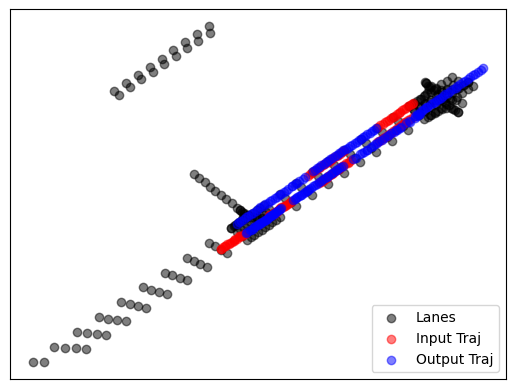
\includegraphics[width=0.8\textwidth]{sample.png}
    \caption{Red indicate input trajectories and blue indicate output trajectories}
    \label{fig:sample}
  \end{figure}
  \item We will be analysing the datasets according to the city they are recorded in for better understanding of the distribution
  of the data. The dataset is recorded in two cities namely Miami and Pittsburgh. The heatmap of the distribution of the input
  data for the two cities are shown in the figure. Figure \ref{fig:heatmap_pitt} shows the heatmap for the city of Pittsburgh and Figure \ref{fig:heatmap_miami} shows the heatmap for the city of Miami.
\begin{figure}[h]
  \centering
  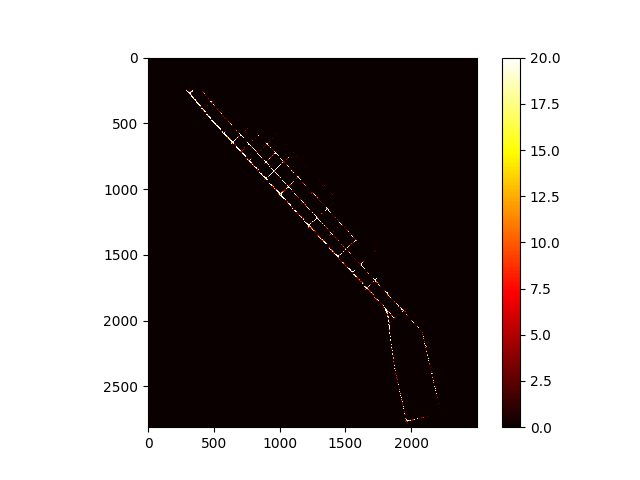
\includegraphics[width=0.8\textwidth]{pitt_inp.png}
  \caption{Heatmap of the distribution of the input data for the Pittsburgh}
  \label{fig:heatmap_pitt}
\end{figure}
\begin{figure}[h]
  \centering
  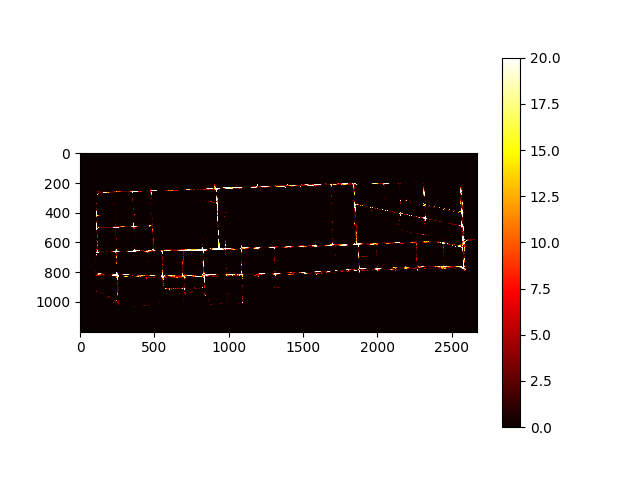
\includegraphics[width=0.8\textwidth]{miami_inp.png}
  \caption{Heatmap of the distribution of the input data for the Miami}
  \label{fig:heatmap_miami}
\end{figure}
  \item We simply plotted the world frame coordinates of all the agents in the dataset for inputs and outputs seperately.
  For the city of Pittsburgh, many of the input coordinates is near the intersection. This shows that the agent can either go straight or take a turn.
  This can be deduced from the output distribution, which shows that we have enough samples (more than moving straight on the intersection) so that model would consider the turn and
  not overfit on agent going straight.
  \item For the city of Miami, the input and output distribution is concentrated on the straight road. This tells
  us that the agent can either move straight or change the lanes. The classificstion of these cases is explained in the next steps.
  \item From plotting the trajectories seperately for each agent we observed that there are four major cases for the agent: moves straight, is parked or at rest, taking a turn
  and finally changing the lanes. The figure shown below shows the distribution of the four cases for both the cities seperately.
  \item To check whether a particular agent taking turn we check the angles made by the trajectories of the agent. Here threshold angle for a turn is taken as 
  60 degrees. Approach to classify the vehicle at rest is straightforward, we simply look through the velocity data of the agent. 
  To classify agent moving in a straight line we try to fit the trajectory of the agent to a line and check the error. If the error is less than a threshold value
  it is traversing in a straight line. Finally, all the samples which does not fall in any of the above three categories are classified as changing lanes.
  The information of this classification is summarized in the Table \ref{tab:classification}.
  \begin{table}
    \centering
    \begin{tabular}{|c|c|c|c|c|}
      \hline
      City & Straight & Turn & Lane Change & At Rest \\
      \hline
      Pittsburgh & 92357 & 1917 & 1247 & 0 \\
      \hline
      Miami &  106420 & 2287 & 1714 & 0 \\
      \hline
    \end{tabular}
    \caption{Classification of the agents}
    \label{tab:classification}
  \end{table}
  \item Since, the data provided is numerical in nature we did not any feature engineering for representation of the data. although as mentioned above we classified the data into four categories,
  this information was used only for analysis and hyperparamter tuning.
  \item As, the 2D pose provided in the dataset is in the world frame, we normalized each of the input and output 2D pose with respect to the first input 2D pose so that we can focus on the 
  patterns of the trajectories rather than the absoluted values. This will help the model to learn the patterns more efficiently. 
  \item We used the city information provided to train the model seperately based on the city. This was done as the distribution of the data is different for the two cities.
  And it would be easy for model to learn the patterns if the data is trained seperately.
  \item Initially we tried to normalize the data in the range of $[0, 1]$ but the model was not able to learn the patterns effectively. This was because the of the vanishing gradient problem. 
  Since, the values of the input and output data were in the range of $[0, 1]$, the gradients were also in the same range resulting in very low loss and small gradients, hence the model was not able to learn the patterns.
\end{itemize}

\section{Deep Learning Model}
As mentioned above we remodeled the given the dataset such that each sample consisted the information about the agent 
to be tracked. We described the preprocessing done on the dataset in the previous section including the normalization, 
transfromation of the coordinate axes and lastly classification based on the cities. Now, we fed the processed data directly to the model.
We tried two main models in this project. The first model is a Multi-Layered Perceptron (MLP) model and the second model is based on LSTM architecture.
\begin{itemize}
  \item For the MLP, we followed a straightforward approach as the input and output data are numerical in nature. And as 
  we are only using 2D poses (and velocities in some cases) the size of input and output is fixed. We vectorized both the input and output data (processed) and fed it to the model.
  \item The model consists of 3 hidden layers with 256, 256 and 256 neurons respectively followed by ReLU activation function. We experimented with both L1 and MSE loss functions and concluded that
  MSE loss was better for training the model (intuitive). But we saw that L1 loss converged faster than MSE Loss, hence, we later used the L1 loss for testing purposes.
  \item For the LSTM based architecture, we remodeled the data such that the input and output data have same shape (19 timesteps). The label consisted of the 2D pose of the agent at the 20th timestep and so on.
  \item The model consists of an LSTM layer with 3 hidden layers with 200 cells in each which is then followed by a MLP with 4 layers with 600, 600, 200 and 2 neurons respectively. The output
  of which is again fed into an LSTM layer which is exactly same as the first one. This architecture is similar to the basic Encoder-Decoder architecture.
  \item We chose the model mentioned above because it is quite effective for sequence to sequence prediction. And as the input and output data is sequential in nature, we thought of using this architecture.
  \item We used the MSE loss function for training the model. We also tried using the L1 loss function but faced similar problem as mentioned for the MLP. Hence, we decided to go with the MSE loss function with Adam optimizer.
  \item We tried using the dropout layer and L1 regularization in the MLP model but it did not help in improving the performance of the model. This might be due to large size of the dataset compared to the number of parameters in the model.
  \item For LSTM model, we used the dropout layer with a dropout rate of 0.2. This helped in improving the performance of the model. As mentioned above, the LSTM was quite dense and hence, the dropout layer helped in regularizing the model.
  \item The model architecture for both the models is shown in the Figure \ref{fig:mlp} and Figure \ref{fig:lstm} respectively.
  \begin{figure}
    \centering
    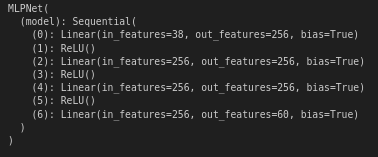
\includegraphics[width=0.8\textwidth]{mlp.png}
    \caption{MLP Model Architecture}
    \label{fig:mlp}
  \end{figure}
  \begin{figure}
    \centering
    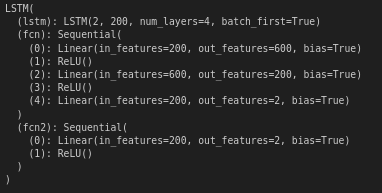
\includegraphics[width=0.8\textwidth]{lstm.png}
    \caption{LSTM Model Architecture}
    \label{fig:lstm}
  \end{figure}
  \item We mainly focused on tuning the batch size, learning rate, number of layers (for MLP model) and number of cells (for LSTM model). We did hyperparameter tuning on a subset of the data (as mentioned above). Other hyperparamters were adopted from literature review.
  The details of the hyperparamaters used are mentioned in the Table \ref{tab:hyperparamters}.
  \begin{table}
    \centering
    \begin{tabular}{|c|c|c|}
      \hline
      Hyperparameter & MLP & LSTM \\
      \hline
      Batch Size & 512 & 256 \\
      \hline
      Learning Rate & 0.001 & 0.001 \\
      \hline
      Decay Rate & 0.95 & 0.95 \\
      \hline
      Optimiser & Adam & Adam \\
      \hline
      Loss & MSE, L1 & MSE, L1 \\
      \hline
      Epochs & 500 & 100 \\
      \hline
      Number of Layers & 3 & 3 + 3 + 3 + 1  \\
      \hline
      Number of Cells & - & 200 \\
      \hline
    \end{tabular}
    \caption{Hyperparamters used for training the model}
    \label{tab:hyperparamters}
  \end{table}
\end{itemize}

\section{Experiment Design and Results}
The details of the implementation of a deep learning model and the analysis done to arrive at a particular model is mentioned in this section.
\subsection{Experimental Setup}
\begin{itemize}
\item We used mainly two devices for this project. The device used for small testing purposes and deciding on minute implementation is 
laptop with 8GB RAM and 12th Gen Intel(R) Core(TM) i7-1255U. For training the final model we used the device provided by the 
UCSD Datahub platform which contains Intel(R) Xeon(R) Gold 6230 CPU @ 2.10GHz, 16GB RAM and 1 GPU, GeForce RTX 2080 Ti with 11GB memory. 
\item We used the Adam optimizer with learning rate of 0.001, decaying at each step with rate of 0.05. We did hyperparameter tuning on a subset of the data.
As mentioned above we classified the data into four categories of the motion of the agent. So, we sampled few samples from each of the four categories to form a subset of the data for hyperparameter tuning.
The values with which we experimented were chosen based on the literature review done in the past.
\item We also experimented on various batch size. For testing purposes we used batch size of 32 on the subset of training data and trained 
the model for 100-500 epochs (500 for MLP and 100 for the LSTM) for the loss to converge. For the final model we used batch size of 512 and trained the model for 500 epochs (or early stopping) which used up lot of resources and time.
\item MLP takes about 6 seconds to go over the complete training data for one epoch whereas, LSTM takes about 200 seconds to go over the complete training data for one epoch.
\item As mentioned above for the MLP we predicted the 2D pose of the agent as a vector of length 60, whereas, for the LSTM we broke the complete trajectory into subsequences and predicted the last term of the subsequence. Hence, we had to remodel the data for this purpose.
\item The number of parameters used in the MLP model is about 6.5 million whereas, the number of parameters used in the LSTM model is about 1 million.
\end{itemize}

\subsection{Results}
\begin{itemize}
  \item The training and validation loss for models are mentioned in Figures \ref{fig:mlp_error} and \ref{fig:lstm_error} respectively.
  \begin{figure}[h]
    \centering
    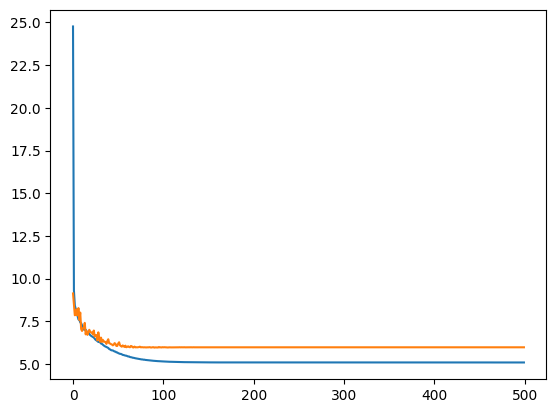
\includegraphics[width=0.8\textwidth]{mlp_error.png}
    \caption{MLP Training and Validation Loss}
    \label{fig:mlp_error}
  \end{figure}
  \begin{figure}[h]
    \centering
    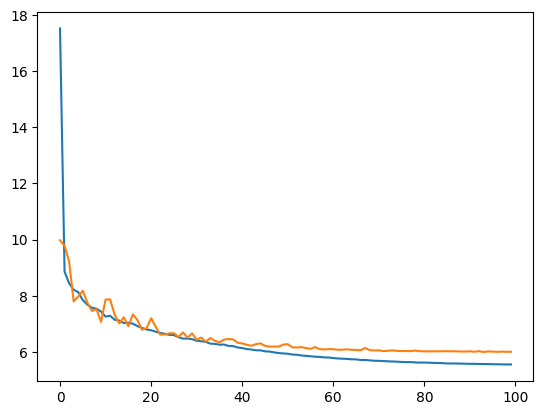
\includegraphics[width=0.8\textwidth]{lstm_error.png}
    \caption{LSTM Training and Validation Loss}
    \label{fig:lstm_error}
  \end{figure} \\
  \item Few training examples are shown in the figures below (Red refers to the input trajectory, Blue refers to the predicted trajectory, and Green refers to the ground truth trajectory):
  \begin{figure}[h]
    \centering
    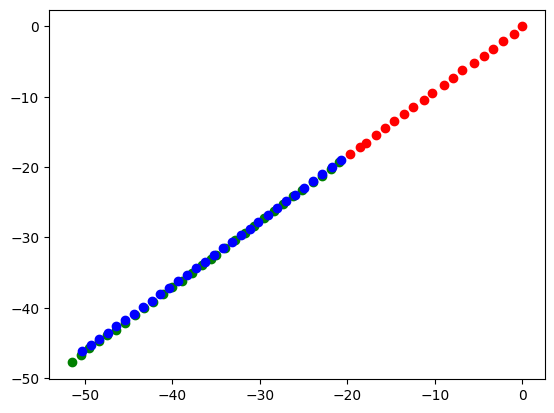
\includegraphics[width=0.8\textwidth]{mlp_1.png}
    \caption{MLP Training Example}
  \end{figure}
  \begin{figure}[h]
    \centering
    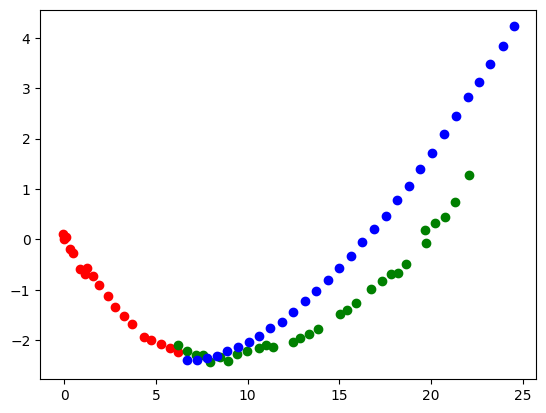
\includegraphics[width=0.8\textwidth]{lstm_1.png}
    \caption{LSTM Training Example}
  \end{figure}
  \begin{figure}[h]
    \centering
    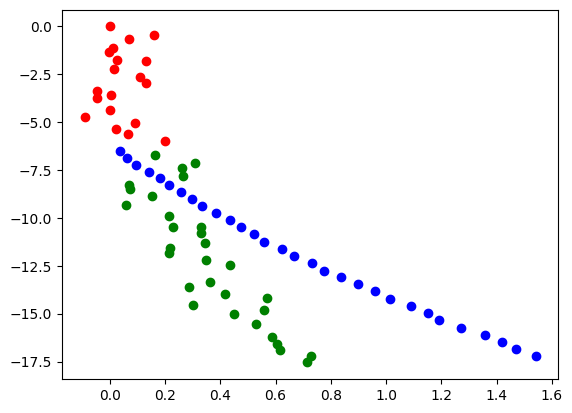
\includegraphics[width=0.8\textwidth]{mlp_2.png}
    \caption{MLP Training Example}
  \end{figure}
  \begin{figure}[h]
    \centering
    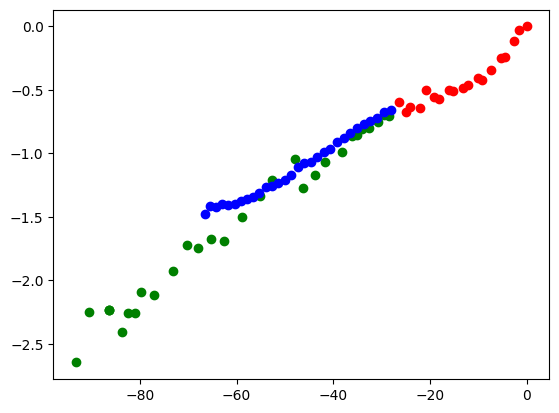
\includegraphics[width=0.8\textwidth]{lstm_2.png}
    \caption{LSTM Training Example}
  \end{figure}
  \begin{figure}[h]
    \centering
    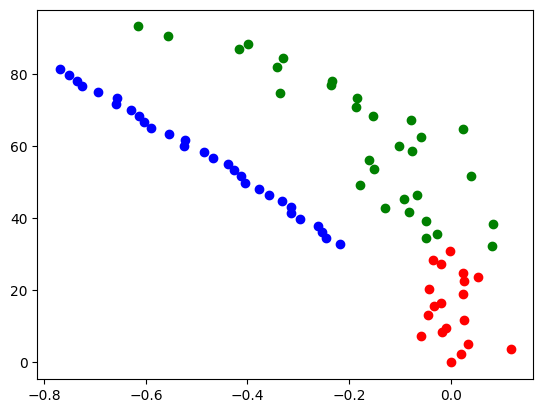
\includegraphics[width=0.8\textwidth]{mlp_3.png}
    \caption{MLP Training Example}
  \end{figure}
  \begin{figure}[h]
    \centering
    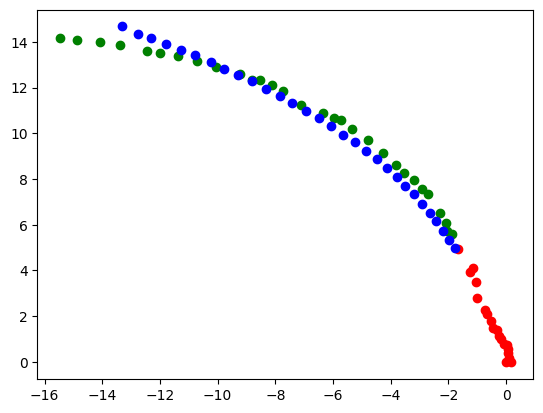
\includegraphics[width=0.8\textwidth]{lstm_3.png}
    \caption{LSTM Training Example}
  \end{figure}
  \begin{figure}[h]
    \centering
    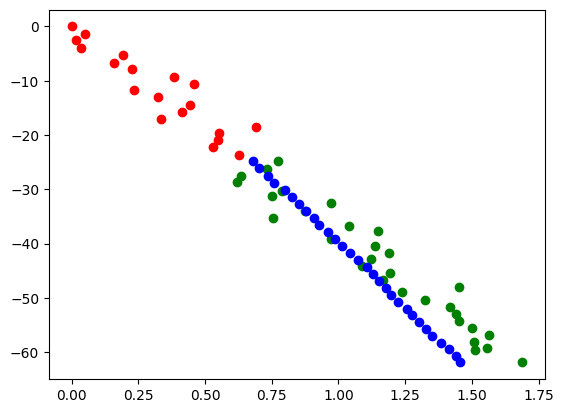
\includegraphics[width=0.8\textwidth]{mlp_4.png}
    \caption{MLP Training Example}
  \end{figure}
  \begin{figure}[h]
    \centering
    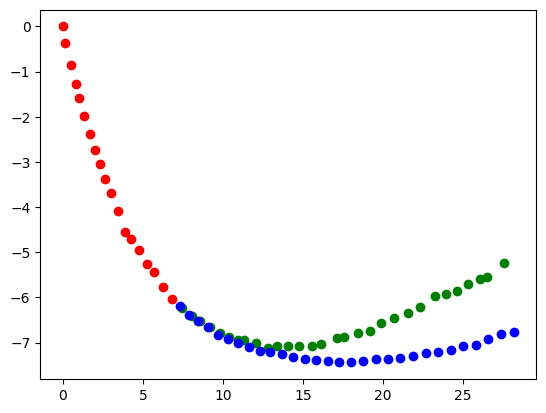
\includegraphics[width=0.8\textwidth]{lstm_4.png}
    \caption{LSTM Training Example}
  \end{figure}   \\
  \item Current ranking (Awies Mulla) - 10th on the leaderboard. Final MSE - 628.
\end{itemize}

\section{Discussion and Future Work}
\begin{itemize}
  \item For this project most effective strategy for me turned out to be transformation of the coordinate axes as this step reduced the 
  variance in the data by a large margin and hence, we were significantly able to reduce the MSE.
  \item The other strategy that worked for me was to use the LSTM model. The LSTM model was able to capture the temporal dependencies in the data and hence, was able to predict the trajectory better than the MLP model, hence reducing the MSE by a large margin.
  \item One of bottleneck of this project was when we were training on a MLP model, trying to achieve results which were beyond the capacity of the model. 
  \item We should always start by analysing the data and building a mini dataset which should be used for most of the analysis. Later, train a model on the complete dataset once we get satisfactory results on the mini dataset.
  Understand the bottleneck of the model with respect to data and one's implementation.
  \item We would later like to experiment with Attention mechanism and see if it improves the performance of the model. We would also like to try implementing 
  models openly available in the literature and see if we can improve the performance of the model.
  \item One of main idea with which we would like to experiment is trying to incorporate the Kalman Filter with the output of the model.
  The output from the could be labeled as the observations obtained and use the Euler's discretized equations of motion as the motion model to predict the trajectory.
  We ae confident that this would improve the performance of the model significantly. We were not able to implement this idea due to time constraints.
\end{itemize}


\end{document}